\documentclass[12pt]{article}
\usepackage[margin=1.0 in]{geometry}
\addtolength{\topmargin}{.25in}
\usepackage[utf8]{inputenc}
%\usepackage[T1]{fontenc}
%\usepackage{textcomp}
\usepackage{xcolor,colortbl}
\DeclareUnicodeCharacter{00A0}{~}
\usepackage{amsmath}
\usepackage{graphicx}
\usepackage{caption}
\usepackage{subcaption}
\usepackage{calc}
\usepackage{array}
\usepackage[noend]{algpseudocode}
\usepackage{pifont}
\usepackage{courier}
\usepackage{relsize}
\usepackage{float}
\usepackage{amssymb}
\usepackage{tikz}
\usetikzlibrary{shapes,arrows}
\usetikzlibrary{positioning}
\newcommand{\textapprox}{\raisebox{0.5ex}{\texttildelow}}
%\usepackage{pgfgantt}
\usepackage{hyperref}
\usepackage{upquote}
\usepackage{natbib}
% Natlib ignore hack start
\let\bibhang\relax
\let\citename\relax
\let\bibfont\relax
\let\Citeauthor\relax
\expandafter\let\csname ver@natbib.sty\endcsname\relax
% Natlib ignore hack end
%\usepackage[style=numeric]{biblatex}
\usepackage[backend=bibtex,style=numeric,sorting=none]{biblatex}
\addbibresource{refs.bib}
\newcommand{\HRule}{\rule{\linewidth}{0.5mm}}
\usepackage{hyperref}
\newcommand{\Green}{\tikz\draw[green,fill=green] (0,0) circle (1 ex);}
\newcommand{\Lime }{\tikz\draw[brown,fill=brown] (0,0) circle (1 ex);}
\newcommand{\Blue}{\tikz\draw[blue,fill=blue] (0,0) circle (1 ex);}
\newcommand{\Yellow}{\tikz\draw[yellow,fill=yellow] (0,0) circle (1 ex);}
\newcommand{\Red}{\tikz\draw[red,fill=red] (0,0) circle (1 ex);}
\renewcommand*\contentsname{Table of contents}
\newcommand{\scm}{\texttt{scan\_for\_matches} }
\newcommand{\scmp}{\texttt{scan\_for\_matches.} }
\newcommand{\sfm}{\texttt{scanfm} }
\newcommand{\sfmp}{\texttt{scanfm.}}
\newcommand{\pu}{PU }
\newcommand{\pus}{PU's }
\newcommand{\pusp}{PU's. }
\newcommand{\pup}{PU. }
\definecolor{listinggray}{gray}{0.9}
\definecolor{lightgreen}{HTML}{E8FFE1}
\definecolor{lightred}{HTML}{FFE1E1}
\usepackage{listings}
\lstset{
	language=C,
	literate=
		{æ}{{\ae}}1
		{ø}{{\o}}1
		{å}{{\aa}}1
		{Æ}{{\AE}}1
		{Ø}{{\O}}1
		{Å}{{\AA}}1,
	backgroundcolor=\color{listinggray},
	tabsize=3,
	rulecolor=,
	basicstyle=\scriptsize,
	upquote=true,
	aboveskip={1.5\baselineskip},
	columns=fixed,
	showstringspaces=false,
	extendedchars=true,
	breaklines=true,
	prebreak =\raisebox{0ex}[0ex][0ex]{\ensuremath{\hookleftarrow}},
	frame=single,
	showtabs=false,
	showspaces=false,
	showstringspaces=false,
	identifierstyle=\ttfamily,
	keywordstyle=\color[rgb]{0,0,1},
	commentstyle=\color[rgb]{0.133,0.545,0.133},
	stringstyle=\color[rgb]{0.627,0.126,0.941},
}
\begin{document}
\begin{titlepage}
\begin{center}

\textsc{\Large Bachelor Thesis \\[0.2in]
University of Copenhagen, DIKU}
\HRule \\[0.4cm]
\textsc{\LARGE \bfseries Optimized pattern matching in genomic data}\\[0.1cm]
\HRule \\[1.2cm]
\textsc{\large Martin Westh Petersen - mqt967 \\ Kasper Myrtue - vkl275 \\ -\\
Supervisors: \\ Rasmus Fonseca \\ Martin Asser Hansen}\\[1.0cm]
\end{center}
\begin{center}
\vfill
{\large 8. June 2015}
\end{center}
\end{titlepage}
\tableofcontents \newpage
\section{Introduction}
\nocite{*}
Analysis and research of genomic data such as DNA is beneficial in a variety of fields for example medicine, where
scientists are now able to identify the genes responsible for causing genetic diseases like 
Alzheimer's disease.~\cite{gen} \\ \\
DNA consists of two biopolymer strands that coil around each other forming a double helix. The two strands
connect along the way, binding pairs of molecules called nucleobases. There are four different nucleobases, called
guanine (G), adenine (A), thymine (T), cytosine (C). They bind to each other in complementary pairs, T binds with A and
G binds with C.~\cite{dna} \\ \\
What holds the genetic information in DNA is the sequence of nucleobases along the strands, and thus sequencing DNA
result in a long sequence of these four bases represented as just the letters A,T,G and C. \\ \\
Pattern matching functionality is unavoidable when analyzing and searching for patterns in these sequences, but
huge amounts of data makes it inefficient to manually find these patterns~\cite{gcn}, so there's a need for clever
and efficient software to do this. \\ \\
\scm ~\cite{scm} is a piece of software that serves this purpose, but big improvements in performance can be made.
On top that, the code is poorly documented, lacks version control and is hard to read and maintain. \\ \\
Our goal is therefore to implement a documented program with version control 
that can search for patterns in large data files consisting of a letter sequence
with letters from the alphabet A,T,C and G, with guaranteed correctness
and high speed, but using the same complex way of defining patterns as \scmp 
\section{Methods}
\subsection{Defining patterns in \scm}
\scm provides a simple and limited domain-specific language for defining patterns to look for in a text file consisting
of a specific alphabet, e.g. the four letters (A, T, C and G) representing bases in a DNA sequence. \\ \\
The language revolve around a basic building block called the pattern (\pu) which can take different forms
and be used in combination to define an overall pattern to search for. \\ \\
Each \pu can either match or not match a sub-sequence of data, but it may be able to match the data in several different ways.
To declare an overall match, \scm has to be able to match each \pu in the given order with a consecutive sub-sequence in the
data. It does so by trying to match the \pus one at a time going left to right with a specific starting position in data. 
The algorithm uses backtracking which means that whenever a \pu (call it p2) is not able to match, the algorithm goes back to the
previous \pu (call it p1) to try and find a different match for p1. If successful the algorithm continues to p2 again. The
different way of matching p1 may have resulted in a different starting position for p2, which may enable p2 to 
actually find a match this time. If there was not way of finding an overall match the algorithm increments the starting
position for the first \pu and tries again. It continues like this until the end of the data file. \\ \\
\scm offers some features besides the use of just \pusp These features apply to the \pus and alter their criteria
for matching.
The different formats of \pus and some of the extra features are described in the list below.
\begin{itemize}
\item a sequence \pu consists of a specific sequence of letters from the alphabet which will
only match if the compared sub-sequence in data has the exact same letters in the exact same order as the 
sequence \pu. \\ \\
Example of sequence \pu : \texttt{AGGT}
\item A range \pu consists of 2 positive integers separated by three dots, where the first integer is less than or
equal to the second. The \pu matches any combination of
letters from the alphabet that has a length that is equal to one of the integers or any integer in between those integers. \\ \\
Example of range \pu : \texttt{4...8} which matches any letter combination of length 4,5,6,7 or 8.
\item A variable can be assigned either a range \pu or a sequence \pu for later reference. The variable is specified by 
any user defined name
followed by an equality symbol and then followed by a range \pu or a sequence \pup \\ \\
The range or sequence PU functions normally, but at run-time the letter combination that it matches
in data is saved, and one can reference it in a later \pu by simply writing the name of the variable. That is a
reference \pu and functions as a sequence \pu but uses the specific saved 
letter combination to match with. \\ \\
Example using variable/reference \pu : \texttt{p1=4...6\; ATG\; p1}, where
the first \pu is the range \pu with added variable functionality, 
and the third being the reference \pu that is linked to the first \pup
\item Any sequence or reference \pu can be made flexible by allowing a number of specified
single-letter edits; insertions, deletions and mismatches. \\ \\
A mismatch allows one letter from the \pu to match one letter in the data even though they're not the same.
An insertion allows for a temporary insert of one letter in the \pu letter combination that matches one letter in
the data, thus lengthening the \pup A deletion allows for temporarily ignoring one letter in the \pu letter combination
and jumping straight the next letter, thus shortening the \pup \\
An example of each edit is shown in Figure 1. \\ \\
Example using single-letter edits : \texttt{p1=TGTGTCT[1,0,3]\; ATTCC[1,1,2]\; p1[2,2,2]} 
where the first sequence \pu is allowed 1 mismatch, 0
deletions and 3 insertions, the middle sequence \pu is allowed 1 mismatch, 1 deletion and 2 insertion 
and the reference \pu is allowed 2 of each.
\item Putting a $\sim$ in front of a reference \pu means that \scm tries to match the reverse 
complement of the letter-sequence saved in the variable. 
The reverse complement of a letter sequence is a sequence of same length, where it has been reversed and every letter
is substituted with its complementary counterpart (A swaps with T and vice versa, G swaps with C and vice versa).\\ \\
Example using the $\sim$ feature : \texttt{p1=3...4\; GG\; $\sim$p1} would match the data sub-sequence:
"TCACGGGTGA" since "GTGA" is the reverse complement of "TCAC".
\item Ambiguous letters~\cite{ambi} are letters other than the standard letters of the used alphabet. These letters are used
in sequence \pus to allow matching with one of multiple of the standard letters in the alphabet.
In \scm the letter "Y" in a \pu matches either a "C" or a "T" in data, a "D" matches either "A" or "G" or "T" 
and "N" matches any of the standard letters. There is a letter for each different combination of the
four standard letters. \\ \\
Example using ambiguous letters : \texttt{CYDTDNA} matches the sub-sequence "CCGTACA" in data.
\end{itemize}
The list above explains what we have found to be the core features of \texttt{scan\_for\_matches}, 
but other features are available as well. Here are some of them: 
\begin{itemize}
\item A logical "or" between \pus or sets of \pus, e.g. "(\texttt{AGGT} \text{\textbar} \texttt{CCCC})", or  \\
"(\texttt{p1=3...6 TG ~p1[1,0,4]} \text{\textbar} \texttt{p1=3...6 AAA ~p1[2,2,0]})"
allows either of the two sides of the \text{\textbar} to match.
\item Custom pairing rules can be defined, with which the user can define custom letter pairings of in the given
alphabet, instead of the standard rules (A pairs with T and C with G). \\
\end{itemize}
\begin{figure}[H]
\begin{center}
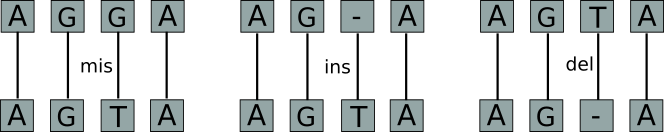
\includegraphics[scale=0.6]{Diagrams/midex.png}
\end{center}
\caption{\textit{The top character sequences are the patterns and the bottom the data. In the first example the G is simply
substituted for a T. In the second example the pattern is AGA but matches the sub-sequence AGTA in data by insertion of a
T. In the third example the pattern AGTA matches the data AGA by deleting the T.}}
\end{figure}
\subsection{Backtracking}
Finding a match between data and a \pu with allowed edits often requires trying 
different combinations of uses of the edits, and \emph{backtracking} is a sort of algorithm that offers this functionality.
Backtracking is the foundation for string search in \scm and in our re-implementation. \\ \\
An implementation similar to
\scm that allows complex patterns to be defined by separable \pus would often require more than just finding \textit{one}
match for a particular \pu with allowed single-character edits. One possible combination of the single-character
edits used to find a match for one particular \pu may result in a valid match of the whole pattern, 
where other combinations that makes a particular \pu match, may prevent a whole match from being possible.
It is therefore necessary for our particular \pu to be able to find more than one way to make a valid match (if these are
possible). Consider the example in Figure 2 where the pattern is \\ \\
\texttt{CT\; AGCA[2,1,0]\; CG}, i.e. 2 mismatches and
one deletion allowed for the second PU, and the data is \\ \\
"CTAGACGT"
\begin{figure}[H]
\begin{center}
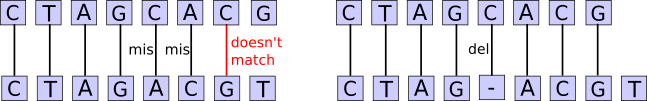
\includegraphics[scale=0.8]{Diagrams/back.png}
\end{center}
\caption{\textit{In the leftmost example the} \pu \texttt{AGCA} \textit{chooses to use 2 mismatches to match the 
data sub-sequence} "AGAC" \textit{and then move on the next} \pup \textit{The next} \pu
\textit{would then have to match it's letters} \texttt{CG} \textit{with the data sub-sequence} "GT"
\textit{which it can't do without edits. The overall algorithm would have to backtrack the the second
} \pu \textit{to try another possible match (if any) to see if that would make a difference. The rightmost example
shows how using a deletion to delete the C in} \texttt{AGCA} \textit{would match data} "AGA" \textit{and
when moving forward to the next} \pu \texttt{CG} \textit{will match} \texttt{CG}}
\end{figure}
\noindent There are two different ways for a \pu to have multiple different matches with a sub-sequence in data. 
Either it's a sequence or reference \pu with allowed mismatches,
insertions and deletions, or it is a range \pup
Whenever backtracking to one of these, another of the possibilities will be chosen and the algorithm continues to the
subsequent \pu again. The amount of checks that the algorithm would need to perform in order to try out
all possibilities grows in an exponential fashion with the number of \pus and the number of different matches each
\pu has. One could visualize this as a search tree structure, 
where each horizontal level of the tree represents a single \pup The different nodes in each horizontal level
then each represent a different way of matching the overall pattern with data until reaching this \pup 
The edges from parent node to children nodes would then represent the different possibilities of matching the given
\pu with the data.
The nodes would have varying number of branches since \pus have a varying number of ways to match with a give data sub-sequence.
The height of the tree would also vary because which branch is chosen may affect what 
possibilities the subsequent \pu has, and the final \pu may not be reached with every combination. \\
Consider the example in Figure 3 where the pattern is \\ \\
\texttt{AGC[1,1,0]\; TCT[0,1,0]\; TG $<$more} \texttt{PUnits}$>$ and the data \\ \\
"ACCTCTTG$<$more data$>$" \\ \\
Using a deletion to match \texttt{AGC} with "ACC" turns out to be the "wrong" way to go down the tree. This path only
goes down 2 levels in the tree before it becomes impossible to go further. Choosing a mismatch to match \texttt{AGC} with "ACC"
and then matching \texttt{TG} with "TG" without using edits lets us further down the tree (and possibly to the last PU). \\
\begin{figure}[H]
\begin{center}
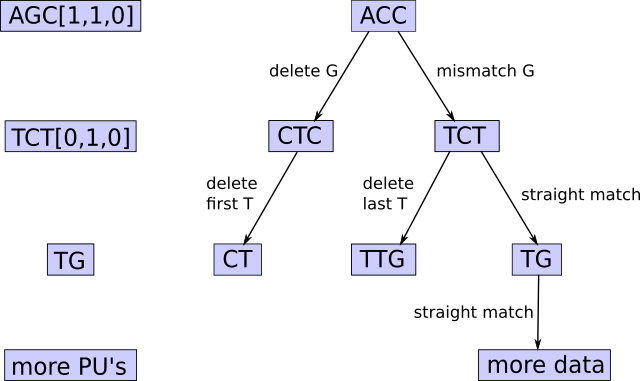
\includegraphics[scale=0.65]{Diagrams/tree.png}
\end{center}
\caption{\textit{The rectangles on the left show the \pus and each horizontal level of the tree represents the \pu 
which is horizontally aligned with it. The letter combination inside each node in the tree shows the part of the data sequence
that the given \pu tries to match with. The text attached to each edge says what choice of use of edits was made 
in order to match.}}
\end{figure}
\noindent It may be that not every path down the tree reaches the last \pu so even though the number of combinations that 
should possibly be tried grows exponentially, it can often times be determined before
reaching the bottom of the tree whether that particular way down is possible or not and if not, the combination does
not have to be checked all the way to the end. \\ \\
The worst case running time would still be exponential since it is possible for a pattern that no possible choice of match
for any \pu would prevent any of the following choices, i.e. the tree would have a homogeneous height, and
all the nodes would have their respective maximum amount of child nodes. \\ \\
Many of the sub-paths in a tree like this may yield the same result on the sub-path's end node, i.e. at a horizontal
level in the tree there may be several identical nodes, and the children of these identical nodes will of course be
identical as well, so when counting towards the number of \emph{different} overall matches, only one of these identical
branches should be considered. \\ \\
Let us define the function $children(\pu)$ to take the a \pu as input and return the amount of possible matches with	
\textit{different lengths} on any data, that the input \pu can have.
In case of mismatches insertions and deletions, the number of characters a match can differ is determined by 
the sum of the insertions (use of these makes the match longer)
and the deletions (use of these makes the match shorter). The last option is using none of the insertions or deletions which
result in yet another match length. \\ \\
If it's a range \pu then the number of different lengths are given by the size of the interval. \\ \\
$children(PU)=
\left\{
\begin{array}{ll}
(PU.max - PU.min) + 1 & \mbox{if } PU=Range \\
PU.insertions+PU.deletions+1 & otherwise 
\end{array}
\right.$
 \\ \\
Let $p$ be a pattern and $p[i]$ be the i'th \pu in $p$, and let $n$ be the number of \pus in $p$,
then the amount of combinations of the different matches of the \pus would be $comb(p)$ \\ \\
$comb(p,n)=\mathlarger{\mathlarger{\prod}_{i=1}^{n}\;children(p[i])}$ \\ \\
Consider the pattern \texttt{AGGT[0,1,1]\; 4...5\; TTCTAA[0,2,1]} called $p1$: \\ \\
$comb(p1,n)=\mathlarger{\mathlarger{\prod}_{i=1}^{3}\;children(p1[i])}= \\ \\
children(\texttt{AGGT[0,1,1]})\;\cdot \;children(\texttt{4...5})\;\cdot \;children(\texttt{TTCTAA[0,2,1]})=
3\cdot 2\cdot 4=24$ \\ \\
A total of 24 leaves on the tree. \\
As mentioned this is the maximum amount of checks that would need to be performed in order to determine if there is a 
possible match at a specific starting position in the data. Even if a tree has a homogeneous 
height, the probability of checking the correct branch lastly is low.
The average actual running time of an algorithm that uses these principles would therefore be significantly better, 
but worst case is: \\ \\
$comb(p,n)$ given a pattern $p$ and the the number of \pus $n$ in that $p$.
\subsection{Flow of \scm}
\scm uses backtracking functionality~\cite{back} on two different levels to find the matches. 
One is the outer backtracking system that backtracks between \pus, and the other is a backtracking algorithm
for matching a single \pu if it has been allowed any mismatches, insertions or deletions. \\ \\
\scm has an outer backtracking system that controls the flow of the outer pattern match, i.e. decides whether to
move forward to the next \pu if the current \pu matched, or backtrack to the previous \pu if there was no match.
When backtracking to a previous \pu the next possibility (if any) for matching is chosen and the algorithm moves
forward again. This problem would normally be solved with recursion and/or loops, but \scm uses GOTO statements which has 
both pros and cons. \\
\begin{figure}[H]
\begin{center}
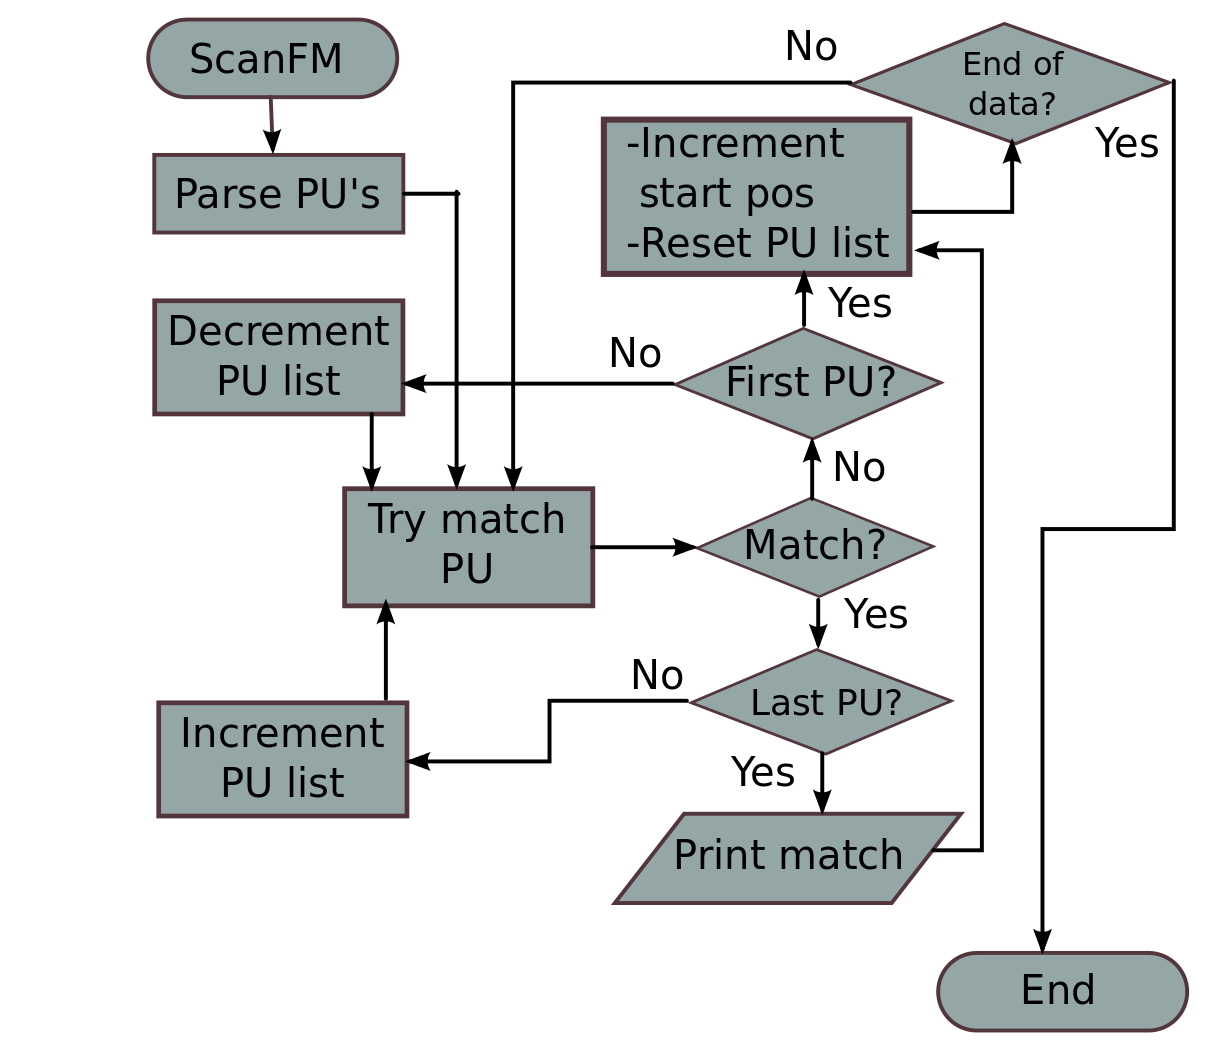
\includegraphics[scale=0.4]{Diagrams/ScanfmFlow.png}
\end{center}
\caption{\textit{Simplistic flow chart of} \scmp \textit{The blue rectangles indicate a process being executed, 
the purple diamonds indicate decisions being made, the green rounded rectangles indicate start and end of the program
and the orange parallelogram indicates output.}}
\end{figure}
\noindent The use of GOTO statements avoids some of the risks associated with the use of recursion like stack overflow. 
How deep the recursion would go would depend on the size of the pattern, and it would therefore be hard to control and
unsafe to use with respect to unwanted termination. Analyzing the possible depth of recursion and rejecting a queried search
if too deep is hardly an option, as it may be necessary to find these large patterns. \\ \\
Even though the use of GOTO statements uses a controllable fixed amount of
memory, it is not necessarily safe. The big con is the missing modularity and structure. 
It is very easy to make a mistake when creating or maintaining that sort of code
(as \scm is a great example of)
because the responsibility is not partitioned into functions or classes that can be unit-tested and proved to work.
Every variable is defined in a global scope and has to be managed as such, which is very prone to error. With every
jump back and forth between the GOTO's all variables and flags must be set just right or the behavior of the program
is undefined. 
One variable being set wrongly due to a particular input and searching in a particular part of the data may 
escalate to either deliver wrong matches or just terminate. \\ \\
Figure 4 shows the overall flow of finding patterns in \scm by backtracking back and forth between the PU's. When
a match is found it is printed to the user, the list of \pus is reset to start with the first \pu and the 
starting position in data is incremented accordingly so the search for other matches can continue. \\ \\
The other backtracking system happens internally in the pattern matching of a single \pu if that \pu has allowed
mismatches, insertions and deletions. Figuring out a way to utilize the allowed edits to possibly find a match, requires
trying out a lot of combinations so this part of the program is the most computationally heavy. 
\subsubsection{Multi-level backtracking}
Sequence or reference \pus that has allowed mismatches, insertions or deletions are handled in a very specific way by \scmp
Starting from left going right in the \pu
and data, the algorithm greedily matches as many characters as possible without using allowed edits.
Every time a character doesn't match, \scm spends an edit and uses a stack structure to keep track of which
kind of edit should be tried next at this point in the sub-sequence, in case the rest of the \pu doesn't match and need to
backtrack to this spot. The different edits are tried in the following order: mismatch, deletion, insertion, i.e.
if a character doesn't match the character in data and this spot was approached from the left (not backtracking)
then a mismatch is used. When backtracking to this spot then an insertions is tried, and if that failed as well further along 
in the \pu a deletion is tried. \\ \\
By only using edits when necessary, \scm exploits the property of \emph{dominance relation}.~\cite{dom}
Dominance relation can be applied in many combinatorial problems, and allows for some of the solution
space of a problem to be dismissed as it can never be an optimal solution due to a "dominant" other part of the solution space. 
A good example is the classic knapsack problem~\cite{knap}; 
Given a set of items that each has a weight and value assigned to them,
and then a bag that can contain items up to a certain weight limit, determine how many of the different items to
include in order to maximize the total value but keeping the weight under the limit. If one of the items $I_1$ weighs
X and is worth Y, but a combination of other items (say $I_2$ and $I_3$) weighs less than X and is worth more than Y, 
then item $I_1$ can never be part of an optimal solution to this problem, since in any solution that contains $I_1$, 
one could substitute $I_1$ for $I_2$ and $I_3$ and get more value without breaking the weight limit, in which case the 
original solution containing $I_1$ was not optimal. \\ \\
The naive way of trying to fit a \pu to a sub-sequence in data using edits would be trying out every permutation of the edits
applied on the characters, even those which actually matched the data. The number of permutations would be very large,
so \scm uses dominance relation to rule out many of the permutations and speed up the search. \\
In other words, whenever \scm
encounters a character that matched the character in data, spending a mismatch, insertion or deletion is never
considered and never tried out, because the property of dominance relation promises that spending an edit
here is not necessary for finding a match. 
Figure 5 shows an example of a match between pattern and data that uses edits where it was not required,
and how one can transform this into a match that uses its first edit at the first mismatching characters.
The pattern is \texttt{ATTTTG[0,2,0]} and the data is "ATTG".
\begin{figure}[H]
\begin{center}
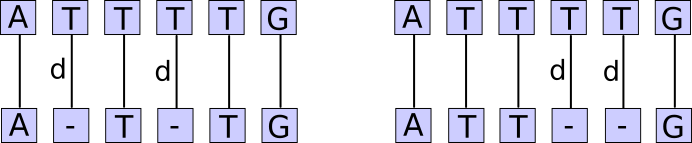
\includegraphics[scale=0.6]{Diagrams/shunt.png}
\end{center}
\caption{\textit{The leftmost example uses its two deletions where it was not necessary, and the rightmost example shows
the same match where the use of the deletions have been postponed as much as possible before being used.}}
\end{figure}
\noindent Using dominance relation \scm always finds a match for a \pu if it exists, but when used in combination
with an outer backtracking system that is not enough! \\ \\
The technique described is useful only if the goal is determining if there exist a possible match or not.
With an outer backtracking system it is often times required that several if not all possibilities are tried in
order to find the overall match. Some \pus of the overall pattern may be required to be of a specific length in order to
match the whole pattern, and the only way such a \pu can obtain the required length may very well be using unnecessary
edits. Trying to match a \pu with allowed edits, \scm will always accept the first way of matching, and even if
subsequent \pus fail and we backtrack to this \pu again, the same match with the same length will be found. 
It is therefore not guaranteed that \scm will find all the matches it's supposed to find. In fact every sub-sequence
of data that should match with the pattern, but requires for one or more of its \pus to have a length only
acquirable by using unnecessary edits, \scm will not find!
Figure 6 shows the flow of \scm in pseudocode that illustrates the 
inexhaustive way \scm glues the outer and inner backtracking together.
\begin{figure}[H]
\begin{center}
\begin{algorithmic}[1]
  \Procedure{Scan\_for\_matches}{list$<$PU$>$ PUs, string data}
    \For{int i = 0 to length(data)}
      \If{\Call{matchPUs}{PUs, data, i}}
        \State print i
      \EndIf
    \EndFor
  \EndProcedure \\
  \Procedure{matchPUs}{list$<$PU$>$ PUs, string data, int i}
    \For{j = head(PUs).min\_range to head(PUs).max\_range}
      \If{\Call{findmatch}{head(PUs), data, i}}
        \If{\Call{matchPUs}{tail(PUs), data, i + j}}
          \State \Return true
	    \EndIf
	  \EndIf
    \EndFor
    \State \Return false
  \EndProcedure \\
  \Procedure{findmatch}{PU p, string data, int i}
    \State \Return the endpoint of the first match found using PU p, data and start position i
  \EndProcedure
\end{algorithmic}
\end{center}
\caption{\textit{Pseudocode that shows simplified flow of} \scmp \textit{The .min\_range and .max\_range attributes
contain the minimum and maximum length of a range \pup They are 0 for non-range PU's in which case the loop runs
only once.}}
\end{figure}
\noindent The first procedure handles the traversing through the data. The third procedure finds only one match (and always 
the same) given a PU, data and a starting position, and thus other possible matches with different lengths than the
one found on line 8 will not be tried. Consider the example in Figure 7 where
the pattern is: \texttt{AAA[0,2,0] AT} and the data is "AAAT". Only by using an unnecessary deletion in the first
\pu will the second \pu match. The call on line 8 will return only 3.
\begin{figure}[H]
\begin{center}
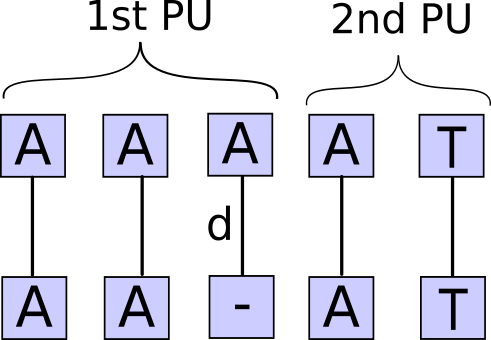
\includegraphics[scale=0.3]{Diagrams/scnfail.png}
\end{center}
\caption{\textit{The top sequences are the \pus and the bottom the data.} \scm \textit{would not find this match!}}
\end{figure}
\noindent Not only does \scm not find matches where unnecessary edits are required, \scm doesn't  
find overall matches that requires a certain combination of uses of edits in a \pu if a match was found for this
\pu using a different combination of edits, and this combination is tried before the one that yields the overall match.
As previously stated the order in which the edits are tried is: mismatches, deletions, insertions, so if
a \pu is allowed 1 mismatch and 1 deletion and can match the data using either one of the two, the match using the
mismatch edit will always be chosen, and if the subsequent \pu requires the first \pu to match 1 character less
in the data (which could have been done using the deletion instead of the mismatch), 
the overall match will not be found by \scm even though it was supposed to. And example of exactly this is shown in
Figure 8, where the pattern is \texttt{AGGT[1,1,0] TCA} and the data is "AGTTCAG".
\begin{figure}
\begin{center}
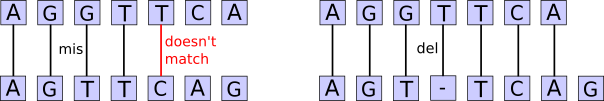
\includegraphics[scale=0.8]{Diagrams/fail2.png}
\end{center}
\caption{\textit{The example on the left shows the way} \scm \textit{would always try to match given the pattern and the data.
The rightmost example shows how to match the first \pu in order to make the whole pattern match.}}
\end{figure}
\subsection{Design}
Our re-implementation of \scm called \sfm is developed in C++ rather than C, which was used to develop 
\texttt{scan\_for\_matches}. We have used C++ classes instead of C structs as the base structure for the PU's. \\ \\ 
Figure 7 shows the class structure of \texttt{scanfm}. The "Sequence" and "Range" classes inherit from the overall
class "PUnit", and the "Reference" class inherit from the "Sequence" class, since a reference \pu works exactly like a 
sequence \pu at run-time when it has collected its letter sequence from either a sequence \pu or a range \pup \\ \\
\sfm has been implemented to support every core feature of \scm as described previously except the one
that allows for a reference \pu to refer to a sequence \pu variable, i.e. \sfm only supports the variable/reference
functionality with variables being assigned range \pusp \\ \\
The syntax for defining patterns in \sfm is the same as in \scm but the pattern is supplied to \sfm through 
the command-line call to \sfmp
\subsubsection{Flow of \sfm}
The control flow of \sfm is similar in idea to \scm but very different in implementation. While \scm uses a case/switch
and GOTO statements, \sfm uses an outer loop to call the "search" function of the \pus and then either
forward to the subsequent \pu on success or backtrack to the previous \pup \\ \\
The control flow of \sfm was originally intended to be very neatly separated into classes and class functions that
didn't encapsulate too much and varying functionality, but in several cases sacrificing a little modularity
was necessary to boost the performance of \sfmp \\ \\
\begin{figure}[H]
\begin{center}
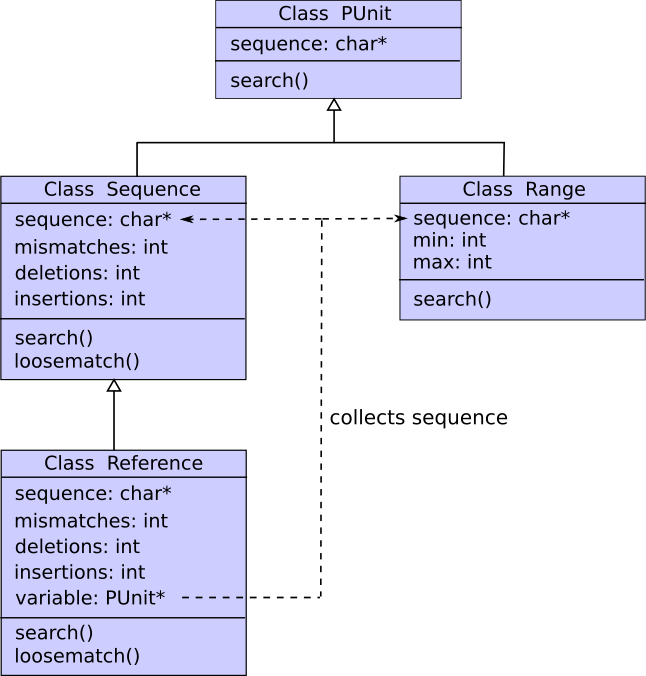
\includegraphics[scale=0.65]{Diagrams/classdia.png}
\end{center}
\caption{\textit{A simplified class diagram which only shows the most important varibles and functions.
There is one generic} \pu \textit{class called "PUnit". This class holds a lot of the common variables
and flags that are needed no matter what kind of} \pup
\textit{
Each class (except the "PUnit" class itself) defines the method "search", which searches for a match given a start position. 
The function "loosematch" is used for trying to find a match when single-character edits are allowed.}}
\end{figure}
\noindent As an example, it was originally intended that an outer loop traversed the data file, 
and for each starting position called the search function of the first \pu object to try to match
at that starting position and if there was a match, the outer loop would call the next \pu object's search function
with the new starting position obtained from incrementing the old starting position with the length of the first \pu match
and so on. If there was no match, the previous \pu was tried again to find a possible alternate match and if 
the first \pu didn't match, the starting position was incremented with 1. \\ \\
If the first \pu is a sequence \pu most starting positions in a data file will not be able to produce a match
and thus the flow will contain a lot of unnecessary calling and returning of the search function. Consider
an example where the first match for the first \pu is a starting position 4. The flow would proceed as follows: \\
Outer loop calls search function of first \pu with starting position 1. Search function of first \pu doesn't find a match
and returns. Outer loop increments starting position to 2 and calls search function again. Again no match is found
and the search function returns again. This continues until the search starts at position 4. For each starting position
we call the search function, return from the search function and increment the starting position (plus the code
in the search function is executed). \\ \\
Performing an unnecessary call to a function and a return from this function with each starting position amounts
to a lot of extra instructions and decreases the performance significantly on large data files. 
\sfm is designed to avoid this overhead by telling the search function of the given first \pu that it should
continue searching until a match is found, i.e. the first \pu now increase the starting position itself so 
traversing the data file until finding a match for the first \pu now only requires incrementing the starting position
and checking for match. \\ \\
Several optimizations of this sort is implemented in \sfm to speed up the performance, and a structure containing relevant
information is passed back and forth between the calls to the search functions in order to keep track of when special
cases and performance enhancing tricks can be applied. \\ \\
The perhaps most important difference between \scm and \sfm is the way \sfm glues outer and inner backtracking together
to ensure that no possible match is missed, which is shown in simplified pseudocode for \sfm in Figure 10.
Whenever \sfm encounters a sequence of reference \pu with allowed edits
\sfm finds all possible matches for this \pu on the given starting position in data. The different
lengths of the matches are saved in a list such that each length only occur once in the list. For example, if 
there are 6 ways for the \pu to match the data and the lengths of the matches are: 5,5,7,6,4,7 then the list would
look like [5,7,6,4] (the order is irrelevant). If the list is not empty (there was at least one match)
\sfm continues to the subsequent \pu with the new starting position being first element in the list. If at some
point \sfm backtracks to this \pu the next element in the list is chosen for the new starting position and \sfm
continues to the subsequent \pu again and so on. Creating the list of lengths \emph{does} take into account lengths reached using
unnecessary edits so the \pu \texttt{AAA[0,1,1]} on data "AAAG" would produce a list of lengths [2,3,4]. \\ \\
In this way \sfm makes sure that every possible length of match with a \pu is tried out before giving up on said \pu
and backtracking. In case of range \pus the different lengths of matches are easier and much faster to calculate, 
they're simply the lengths that lie within the range supplied by the range \pu, i.e. the \pu \texttt{3...6}
would produce a list of lengths [3,4,5,6]. Sequence or reference \pus with no allowed edits produce a list
of lengths with only one element which is the length of the PU, and thus we have covered each type of \pu and ensured
that they all try every possible length of match before backtracking to previous \pusp This is true for every
\pu in the pattern so at any given starting position in data, the procedure \textsc{\small matchPUs} is
guaranteed to find an overall match if one exists!
\begin{figure}[H]
\begin{center}
\begin{algorithmic}[1]
  \Procedure{Scanfm}{list$<$PU$>$ PUs, string data}
    \For{int i = 0 to length(data)}
      \If{\Call{matchPUs}{PUs,data,i}}
        \State print i
      \EndIf
    \EndFor
  \EndProcedure \\
  \Procedure{matchPUs}{list$<$PU$>$ PUs, string data, int i}
    \State list$<$int$>$ endpoints = \Call{match}{head(PUs), data, i}
    \For{ep in endpoints}
      \If{\Call{matchPUs}{tail(PUs), data, ep}}
        \State \Return true
      \EndIf
    \EndFor
    \State \Return false
  \EndProcedure \\
  \Procedure{match}{PU p, string data, int i}
    \State list$<$int$>$ endpoints = [ ]
    \For{each possible match $m$ at starting position i}
      \If{not i + length($m$) in endpoints}
        \State endpoints.append(i + length($m$))
      \EndIf
    \EndFor
    \State \Return endpoints
  \EndProcedure
\end{algorithmic}
\end{center}
\caption{Pseudocode that shows simplified flow of \sfm}
\end{figure}
\noindent Although the pseudocode indicates that \textsc{\small matchPUs} is called for every single starting position
in data, this is not entirely true. If a match is found, the starting position is incremented with the length of 
the match found before continuing the search, effectively ignoring overlapping matches, so the guarantee of the correctness of \sfm can be summed up like 
this: \\ \\
\sfm is guaranteed to find every possible non-overlapping match in given data searching for a given pattern.
\subsubsection{Optimizing character comparison using bitwise operations}
One of the great tricks used in \scm is the use of bitwise operations in performance critical parts of the code.
Comparing single characters is the most used operations and maximizing the speed of this particular operation 
means everything for the performance of the program. Figure 8 shows how \scm transforms every normal C character into
a custom 4-bit code. These 4 bits are used to represent each of the four letters (A,T,C and G) by having a 1 in one of
the slots and 0 in the other three. The letter G for example is represented as 0100. All possible permutations of 
combining these letters are also represented by a permutation of the bit field, e.g.\ the letter V is written in a \pu 
represents either A,C or G and therefore has the bit field 0111 since A is 0001 and C is 0010. \\
Prior to searching, the data input is of course also transformed to 4-bit representations.
When comparing two characters \scm uses the bitwise AND operator and if the result is not 0000 the characters matches. \\ \\
\scm actually stores 4 more bits (left of our 4-bit field) The complementary letter of the letter represented in the rightmost
bit field is stored in the leftmost bit field, e.g. G would look like 0010 0100 although only on of the 4-bit fields would
be used in a comparison. This leftmost bit field is used when comparing a complementary reference \pu instead
of transforming back and forth between the letters every time a complementary \pu is encountered. \\ \\
We are using this exact technique in \sfm to achieve the same optimal way of comparing characters.
\begin{figure}[H]
\begin{center}
\begin{lstlisting}
int build_conversion_tables()
{
    int the_char;

    for (the_char=0; the_char < 256; the_char++) {
        switch(tolower(the_char)) {
          case 'a': \pu_to_code[the_char] = A_BIT; break;
          case 'c': \pu_to_code[the_char] = C_BIT; break;
          case 'g': \pu_to_code[the_char] = G_BIT; break;
          case 't': \pu_to_code[the_char] = T_BIT; break;
          case 'u': \pu_to_code[the_char] = T_BIT; break;
          case 'm': \pu_to_code[the_char] = (A_BIT | C_BIT); break;
          case 'r': \pu_to_code[the_char] = (A_BIT | G_BIT); break;
          case 'w': \pu_to_code[the_char] = (A_BIT | T_BIT); break;
          case 's': \pu_to_code[the_char] = (C_BIT | G_BIT); break;
          case 'y': \pu_to_code[the_char] = (C_BIT | T_BIT); break;
          case 'k': \pu_to_code[the_char] = (G_BIT | T_BIT); break;
          case 'b': \pu_to_code[the_char] = (C_BIT | G_BIT | T_BIT); break;
          case 'd': \pu_to_code[the_char] = (A_BIT | G_BIT | T_BIT); break;
          case 'h': \pu_to_code[the_char] = (A_BIT | C_BIT | T_BIT); break;
          case 'v': \pu_to_code[the_char] = (A_BIT | C_BIT | G_BIT); break;
          case 'n': \pu_to_code[the_char] = (A_BIT | C_BIT | G_BIT | T_BIT); break;
          default:
            \pu_to_code[the_char] = 0;
            break;
        }
        if (\pu_to_code[the_char] & A_BIT)
            \pu_to_code[the_char] |= T_BIT << 4;
        if (\pu_to_code[the_char] & C_BIT)
            \pu_to_code[the_char] |= G_BIT << 4;
        if (\pu_to_code[the_char] & G_BIT)
            \pu_to_code[the_char] |= C_BIT << 4;
        if (\pu_to_code[the_char] & T_BIT)
            \pu_to_code[the_char] |= A_BIT << 4;
    }
...
\end{lstlisting}
\end{center}
\caption{\textit{The function that prepares the conversion table that is used for converting both data and} PU's. 
\textit{The last 8 or so lines of code is where the left 4 bits is being set to the complementary of the letter
represented in the rightmost 4 bits.}}
\end{figure}
\subsubsection{Why not Levenshtein distance?}
The Levenshtein distance between two strings is defined as \textit{the minimum amount of single-character edits required
to change on string into the other.}~\cite{leve} \\ \\
Calculating the Levenshtein distance can be done quite efficiently, at least faster than our implementation calculates
every possible match given the specific three amounts of single-character edits. One could think that a faster 
implementation would be just summing
the number of allowed mismatches, insertions and deletions, calculating the Levenshtein distance between data sub-sequence
and \pu and then comparing to see if the allowed sum was exceeded. This would not be correct since
calculating the Levenshtein distance does not include requirements for the distribution of the different 
single-character edits, it just finds the minimum \textit{sum} of them. \\ \\
If the task at hand is to determine whether two strings are within a maximum allowed Levenshtein distance of each other,
then simply calculating the Levenshtein distance would be enough. 
If however the task is to determine whether one string can be changed into another string with a maximum amount of $X$  mismatches, $Y$ insertions and $Z$ deletions one can \textit{not} simply calculate the Levenshtein distance of the two
strings and compare the number to the sum of the different edits ($X+Y+Z$) since the Levenshtein distance may not live
up to the additional requirements of a maximum of either of the different edits. An example of this is shown in Figure 9. \\
\begin{figure}[H]
\begin{center}
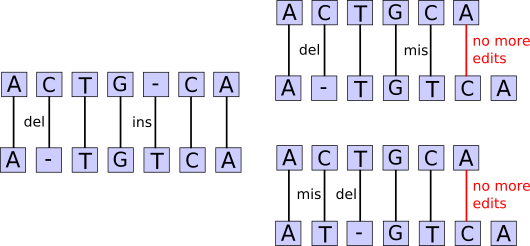
\includegraphics[scale=0.8]{Diagrams/leven.png}
\end{center}
\caption{\textit{The Levenshtein distance between the pattern ACTGCA and the data ATGTCA is 2 
(1 deletion, 1 insertion) as the leftmost example shows. If the pattern is allowed 1 deletion and 1 mismatch, then
the two strings can not match, as the rightmost examples show, even though this also would be a sum of 2 edits.}}
\end{figure}

\subsubsection{Knuth Morris Pratt algorithm}
The algorithm Knuth, Morris and Pratt invented to find substrings in strings in O(m+n) time where m is the substring and n is the string it is looked for in. Where the normal backtracking algorithms gives a worst case time of O(n*m). This can be a huge improvement in cases where there are few different letters and a lot of repetitions, such as most DNA sequences.

The algorithm uses a pre computed sequence, based on the subsequence looked for to determine how far ahead in the string the algorithm can jump when there are close matches.

This could help finding exact matches even quicker in the data, but the real question is whether it could be used to calculate mismatches, insertions and deletions faster, since that is the place in the code the largest improvement is needed.

The Knuth Morris Pratt algorithm has already been formed to calculate a fuzzy match where mismatches are allowed, but a open soudo code is not out there using it for calculating a Levenshtein distance. Calculating the Levenstein distance with this algorithm could potentially give a large improvement in running time.
 

\subsubsection{Optimizing order of \pu matching}
A possible optimization that \scm does \textit{not} exploit, is choosing an order of \pus to be searched for.
Some \pus are more exclusive and rare to find in data than others. Generally the sequence \pu with the most
letters is the \pu that is probably found least times in a big data file. If starting the search by
identifying this rarest \pu the search would save a lot of instructions. \scm starts every search with the 
first \pu in the pattern, and it is therefore often guaranteed to run slower than if it used the other approach.
As Figure 10 shows, this optimization presents a potential huge increase in performance of the program.
\begin{figure}[H]
\begin{center}
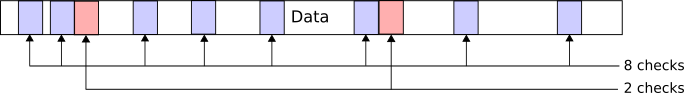
\includegraphics[scale=0.8]{Diagrams/opti.png}
\end{center}
\caption{\textit{A pattern that consists of two} \pus \textit{where the second \\(say}
\texttt{CTCGAATAG}\textit{) is more rare in the data than the first} \pu \textit{(say }\texttt{GGTTCA[1,0,0]}\textit{). 
Searching for the 
second} \pu \textit{first needs three checks (with three additional check afterwards to verify the whole pattern)
while choosing to look for the first} \pu \textit{needs 8 checks (with 8 following checks to verify whole pattern).}}
\end{figure}
\noindent This optimization is introduced in \sfm by calculating a score for each \pu after parsing and before
the search begins. The \pu that received the highest score is called the \emph{optimal} \pu and is 
the \pu that is searched for first. The maximum
distance between the starting position of an overall match and the beginning of the chosen \pu is also calculated, i.e.
the maximum length of each \pu from the start of the overall pattern up to the chosen \pu is summed. The minimum
distance is calculated as well. \\ \\
Whenever a match is found for the chosen PU, the starting position is decremented with the maximum distance and 
\sfm searches for the whole pattern (from the first \pu to the last) in a traditional manner. If there exists an overall
match that contains the match found for the chosen PU, it starts at a position within the maximum distance and 
minimum distance backwards from where the match for the chosen \pu begins, so this traditional match is only carried
out on starting positions within this interval. When the search for an overall match for this interval is done,
the search for the chosen \pu continues throughout the rest of the data. \\ \\
Figure 14 shows how the score of a \pu is calculated. Two factors are considered when finding the optimal PU;
the rarity, i.e. how few times the \pu would match in data, and how quickly \sfm can search for the \pup
Having just a few insertions and/or deletions allowed for a \pu greatly increases the time it takes to look for it,
so \sfm is implemented to never consider \pu containing these as optimal, giving them a score of 0.
\begin{figure}[H]
\begin{displaymath}
   score(PU) = \left\{
     \begin{array}{ll}
       0 & : ins > 0\;or\;del > 0\\
       len-(5+mis+amb) & : mis>0 \\
       len+1000-amb & : len-amb>8 \\
       len-amb & : otherwise
     \end{array}
   \right.
\end{displaymath}
\caption{\textit{ins, del and mis refer to the number of insertions, deletion and mismatches that the given} \pu
\textit{has allowed. The variable amb refers to the number of ambiguous letters contained in the} \pup} 
\end{figure}
\noindent Searching for a \pu that only has allowed mismatches is still slower than for a \pu 
with no edits at all, but it is much
faster than with insertions and deletions. Having any mismatches allowed executes a different and slower part of \sfm
so the difference between no mismatches and any mismatches allowed has a far greater impact on running time than the amount of
mismatches. If any mismatches are allowed the penalty in the score is therefore set quite high to 5, but the number of 
mismatches only counts as a penalty of 1 each. The longer the sequence of the \pu is, the better, so the score
is calculated as the length subtracted any penalties. Ambiguous letters make the \pu less precise and therefore less
rare in the data, so a penalty of 1 i subtracted for each ambiguous letter as well. \\ \\
If a \pu has no allowed edits and the length subtracted the number of ambiguous letters is greater than 8, 
the \pu is considered strict enough to be better than any \pu with allowed edits, giving it a bonus of 1000 points to
ensure that no \pu with allowed edits can surpass it in score. \\ \\
If a \pu that has no allowed edits does not meet the requirement that $len-amb>8$ then a \pu with allowed
mismatches may get a better score. This is done in order to avoid a very short \pu being chosen over a much longer
and rare \pu just because the longer \pu had allowed mismatches, e.g. the \pu\; \texttt{AT}\; should \emph{not} be chosen
over \\
\texttt{GCTAGTCGGCGTCAGTCGTGATAT[2,0,0]}. The former \pu may be faster to search for, but it would match so many
places in data that the number of times the traditional search would be invoked would result in a much bigger
slowdown than the extra time it takes to search for the latter \pup
\subsection{Clean code}
Writing clean code is meant as writing understandable code, that provides overview of the programs
structure. This is necessary when dealing with code that needs to be updated, further developed,
checked for correctness, and debugged. \\ \\
Clean code has been valued when creating \sfm, by dividing responsibilities into classes, and splitting 
those classes into suitable methods. This being said in cases where dividing into different methods 
started to cost running time, the fastest solution has been chosen. This has lead to a larger number of if statements where it can be more difficult to understand the larger picture of certain pieces algorithms. \\ \\
The structure of the \pus has been constructed in a way that it should be possible without to much understanding of the other individual \pus code to create a new \pu. This is so further updating and
development should be as easy as possible. \\ \\
Correctness can be a very strong ally when creating code that needs to be used scientifically, but also
just in cases where correct outputs are important. Splitting the responsibilities into smaller classes 
can make it easier to find faults in the code. It can also be used to create unit tests for each method in
the class. \\ \\
Unit tests in \sfm would further help provide a certainty of correctness to the program, but because
of the complexity of outputs and inputs in \sfm creating unit tests would be very time consuming and
has not been done currently. 
\section{Correctness Test}
In order to show that each \pu works and returns the correct and expected results, they need to be tested individually and in specific combinations. This is done with the use of equivalence classes, this means proving that the edge scenarios of each 
\pu and average scenarios returns the expected result, and by doing so providing a by statistically solid foundation that 
the \pu is correct.
In order to create the largest number of tested features with the least needed tests, the correctness groups has been constructed to create the largest equivalence classes possible. 

\begin{table}[H]
\begin{tabular}{p{2cm}|p{3cm}|p{5cm}|p{4.5cm}}
Feature grouping & Example & Explained & Result  \\ \hline

Simple sequence		& "ACCG"  & A sequence of bases only consisting of basic bases & Empty sequence returns unexpected results\\ \hline

MID sequence 		& "GGGT[2,1,1]" & A sequence og bases with the possibility of mismatches, insertions, and deletions & Pass \\ \hline

Ambiguous base sequence	& "MMNN" & A sequence consisting of only ambiguous bases & Ambiguous base "U" does not function\\ \hline

Ambiguous and basic bases & "MSGGTM" & A sequence consisting of both ambiguous and basic bases & Ambiguous base " does not function\\ \hline

Range & "4...8" & A range of jumps in the data & Range with 0 does not terminate\\ \hline

Simple reference & "p1=3...5 p1" & A reference being made and then searched for  & Ranges with 0 results in wrong found matches\\ \hline

Compleme- ntary reference & "p1=4...7 \textapprox p1" & A reference being made and then the complementary is searched for & Ranges with 0 results in wrong found matches \\ \hline

MID reference & "p1=5...6 p1[2,1,3]" & A reference being made and then searched for with the possibility for mismatches, insertions and deletions & Ranges with 0 results in wrong found matches\\ \hline

MID complementary reference & "p1=3...8 \textapprox p1[1,2,1]" & A reference being made and then the complementary is searched for with the possibility of mismatches, insertions and deletions & Ranges with 0 results in wrong found matches\\ \hline

Multiple \pus & "ACCGMG[1,1,1] 2...8 ACC" & Multiple \pus in a single pattern & Multiple errors described below

\end{tabular}
\end{table}
\subsection{Found errors}
When performing the correctness tests certain errors emerged. None of the found errors where alone
enough to argue that the program is not correct, but if future development ever occurs they would
need attention.
In order to explain what these errors does in a search and how they could be fixed, they are put into
categories:

\subsubsection{Empty sequences}
If a empty sequence occurs in a pattern, the parser should return a error, this does not happen.
This should be changed in the parser, if 2 spaces occurs without anything in between a error message
should be written explaining empty sequences are not allowed.

\subsubsection{Ranges from 0 to 0}
Ranges that does not move the pattern will alone cause a never ending loop. This is not a 
pattern that can be used to find a meaningful match and should not be allowed by the scanfm.
A potent solution would then be to return a error.

\subsubsection{Ranges from 0}
Range from 0 without a \pu after results in a never ending loop. This should not be the case, if a the last
\pu of a pattern is a range from 0, a parse error should occur, since it does not give a meaningful solution
since everything reaching that \pu is true. Another way of handling the error could be to always return successful in the event it reaches the range from 0.

\subsubsection{References with ranges from 0}
In the event a reference contains a range from 0, scanfm returns wrong results, this can not be fixed
by placing a error because it is a valid pattern given by the user. In order to fix this the reference
\pu needs to be able to handle ranges that are 0.



\section{Benchmark comparison}

\newpage
\printbibliography \newpage
\section{Appendics}

\subsection{Correctnes test results}



\subsubsection{Sequence}
To create exhaustive equivalence classes for the \pu sequence, there are multiple scenarios needed to be proven.
A sequence can be exact by having no mismatches, insertions or deletions, it can be loose fitting by having 
mismatches, insertions and deletions or it can be combined with ambiguous bases.
The equivalence class for the exact sequence, needs a test at 0, the smallest possible length and one with multiple bases:
\begin{table}[H]
\begin{tabular}{p{4cm}|p{3.6cm}|p{2.5cm}|p{2.2cm}|p{2.2cm}}
Case 			& Pattern & Data & Expected Result & Result \\ \hline
\rowcolor{lightred}
Empty string		& " " & ACGTNNN & suiting error message & No matches \\ \hline
\rowcolor{lightgreen}
Single base 		& "A" & ANNN & Match at 1 "A" & Match at 1 "A"\\ \hline
\rowcolor{lightgreen}
Multiple bases	& "ACCGT" & ACCGTNNN & Match at 1 "ACCGT" & Match at 1 "ACCGT" \\ \hline
\end{tabular}
\end{table}

The equivalence class for the loose sequence, with mismatches, insertions and deletions has more edge scenarios.
A case with 0 is needed, but in this class there are multiple scenarios for the smallest possible amount of 
mismatches, insertions and deletions, since these are not equivalent they are all needed to be tested. Also the 
combinations of the mismatches, insertions and deletions needs to be tested with both the smallest possible
scenarios and average cases. Finally the scenarios with all of the possible mismatches, insertions and deletions 
being used needs to be tested with both the smallest scenario and a average case.
With deletions and mismatches there are also the scenario where they exceed the pattern length. This also needs to 
be tested.
\begin{table}[H]
\begin{tabular}{p{4cm}|p{3.6cm}|p{2.5cm}|p{2.2cm}|p{2.2cm}}
Case 			& Pattern & Data & Expected Result & Result \\ \hline
\rowcolor{lightgreen}
MID 0			& "ACGT[0,0,0]" & ACGTNNN & Match at 1 "ACGT" & Match at 1 "ACGT" \\ \hline
\rowcolor{lightgreen}
MID 1 miss		& "ACC[1,0,0]" & ACGNNN & Match at 1 "ACG" & Match at 1 "ACG" \\ \hline
\rowcolor{lightgreen}
MID 1 del		& "ATG[0,1,0]" & AGNNN & Match at 1 "AG" & Match at 1 "AG" \\ \hline
\rowcolor{lightgreen}
MID 1 ins		& "ACC[0,0,1]" & ATCCNNN & Match at 1 "ATCC" & Match at 1 "ATCC"\\ \hline
\rowcolor{lightgreen}
MID 2 			& "AGGT[1,1,0]" & ACTNNN & Match at 1 "ACT" & Match at 1 "ACT" \\ \hline
\rowcolor{lightgreen}
MID 2			& "ACGT[1,0,1]" & AGTGTNNN & Match at 1 "AGTGT" & Match at 1 "AGTGT" \\ \hline
\rowcolor{lightgreen}
MID 2 			& "ATTGT[0,1,1]" & ATCGTNNN & Match at 1 "ATCGT" & Match at 1 "ATCGT" \\ \hline
\rowcolor{lightgreen}
MID 3			& "AACGT[1,1,1]" & CAGGTNNN & Match at 1 "CAGGT" & Match at 1 "CAGGT" \\ \hline
\rowcolor{lightgreen}
MID miss multiple & "ACCT[2,0,0]" & ATTTNNN & Match at 1 "ATTT" & Match at 1 "ATTT" \\ \hline
\rowcolor{lightgreen}
MID del multiple & "AGTTT[0,2,0]" & AGTNNN & Match at 1 "AGT" & Match at 1 "AGT" \\ \hline
\rowcolor{lightgreen}
MID ins multiple & "ACGT[0,0,2]" & ACTTGTNNN & Match at 1 "ACTTGT" & Match at 1 "ACTTGT" \\ \hline 
\rowcolor{lightgreen}
MID multiple		& "ACTTT[1,2,0]" & GCTNNN & Match at 1 "GCT" & Match at 1 "GCT"\\ \hline
\rowcolor{lightgreen}
MID multiple		& "TCGAT[3,0,2]" & CGCTTATNNN & Match at 1 "CGCTTAT" & Match at 1 "CGCTTAT" \\ \hline
\rowcolor{lightgreen}
MID multiple		& "TCGGT[0,2,3]" & GGGGGTNNN & Match at 1 "GGGGGT" & Match at 1 "GGGGGT" \\ \hline
\rowcolor{lightgreen}
MID all			& "ATTCCCTT[2,2,1]" & TTCCGTAN NN & Match at 1 "TTCCGTA" or "TTCCGTAN" & Match at 1 "TTCCGTAN"\\ \hline
\rowcolor{lightgreen}
MID more del		& "ATTC[0,6,0]" & CCCCCCNNN & A unknown number of matches not equal to 0
\footnote{Since the code does not specify a order of used deletions, the 
length of the match can be everywhere from 0 to 4, making it hard to predict a result. 
This does not mean that different results can't all be correct. } & Match at 1, 2, 3, 4, 5, and 6 "C" \\ \hline
\rowcolor{lightgreen}
MID more mis		& "ATTCG[8,0,0]" & GGGGTNNN & Match at 1 "GGGGT" & Match at 1 "GGGGGT" \\ \hline
\end{tabular}
\end{table}



In order to create a equivalence class for ambiguous bases in a exact sequence \pu, the same
scenarios as a exact sequence is needed with the addition that all ambiguous bases needs to be
shown to work individually. 
\begin{table}[H]
\begin{tabular}{p{4cm}|p{3.6cm}|p{2.5cm}|p{2.2cm}|p{2.2cm}}
Case 			& Pattern & Data & Expected Result & Result \\ \hline
\rowcolor{lightgreen}
Single ambiguous base & "R"(R is A or G) & ATTGNNN & Match at 1 "A" and 4 "G" & Match at 1 "A" and 4 "G" \\ \hline
\rowcolor{lightgreen}
Ambiguous bases	& "RRGGWW" & AAGGTANN N & Match at 1 "AAGGTA" & Match at 1 "AAGGTA" \\ \hline
\rowcolor{lightred}
All ambiguous bases & "UMMRRWWS SYYKKBBB DDDHHHVV VNNNN" & TACAGATC GCTGTCGT AGTACTAC GACTGNNN & Match at 1 & no Match \\ \hline
\rowcolor{lightgreen}
All ambiguous bases except u & "MMRRWWS SYYKKBBB DDDHHHVV VNNNN" & ACAGATC GCTGTCGT AGTACTAC GACTGNNN & Match at 1 & Match at 1 \\ 
\end{tabular}
\end{table}

In order to make sure that ambiguous bases work correctly with the defined bases, a equivalence class is needed
to show that the smallest mixed scenario and a average scenario works correctly.
\begin{table}[H]
\begin{tabular}{p{4cm}|p{3.6cm}|p{2.5cm}|p{2.2cm}|p{2.2cm}}
Case 			& Pattern & Data & Expected Result & Result \\ \hline
\rowcolor{lightgreen}
Smallest mix		& "AM" & ACAA & Match at 1 "AC" and 3 "AA" & Match at 1 "AC" and 3 "AA" \\ \hline
\rowcolor{lightgreen}
Average mix		& "TTATMTNYY" & TTATATGTC & Match at 1 "TTATATGTC" & Match at 1 "TTATATGTC"
\end{tabular}
\end{table}


\subsubsection{Range}
Range by itself does not make room for a large difference in possibilities, in order to create a 
equivalence class only a few scenarios are needed, the smallest possible cases, a 0 case and a average case.
\begin{table}[H]
\begin{tabular}{p{4cm}|p{3cm}|p{2.5cm}|p{2.5cm}|p{2.5cm}}
Case 			& Pattern & Data & Expected Result & Result \\ \hline
\rowcolor{lightred}
Range from 0...0	& "0...0" & ACCNNN & Suiting error & Never ending loop \\ \hline
\rowcolor{lightred}
Smallest range 	& "0...1" & ACCNNN & Match at all bases & Never ending loop \\ \hline
\rowcolor{lightgreen}
Smallest range without 0 & "1...1" & AGTNNN & Match at 1, 2, 3, 4, 5 and 6 & Match at 1, 2, 3, 4, and 5 \\ \hline
\rowcolor{lightgreen}
Standard case	& "4...9" & AAAAAAAA AANNN & Match at 1 and 5 & Match at 1 "AAAA"
\end{tabular}
\end{table} 



\subsubsection{Reference}
Reference can't be tested and proved correct as a individual \pu since it needs to refer to another \pu
to function. 
In order to make sure the reference \pu works correctly the equivalence class needs to obtain references with and
without another \pu between the refereed \pu and the reference \pu. Both a 0, edge and average case is needed for both
scenarios.
\begin{table}[H]
\begin{tabular}{p{4cm}|p{3cm}|p{2.5cm}|p{2.5cm}|p{2.5cm}}
Case 			& Pattern & Data & Expected Result & Result \\ \hline
\rowcolor{lightred}
0 reference with 	& "p1=0...0 2...4 p1" & ACCCNNN & Match at 1 "ACCC" & Match at 1 "ACCCN" \\ \hline
\rowcolor{lightgreen}
Smallest reference with 	& "p1=1...1 2...2 p1" & ACCANNN & Match at 1 "ACCA" & Match at 1 "ACCA" \\ \hline
\rowcolor{lightgreen}
Standard case with	& "p1=3...5 2...2 p1" & CCCCAACC CCNNN & Match at 1 "CCCCAACCCC" & Match at 1 "CCCCAACCCC"\\ \hline
\rowcolor{lightred}
0 reference without	& "p1=0...0 p1" & TTGTANNN & Undefined & Match at 1 "T", 2 "T", 3 "G", 4 "T", 5 "A", 6 "N", 7 "N", and 8 "N"\\ \hline
\rowcolor{lightgreen}
smallest reference without & "p1=1...1 p1" & AANNN & Match at 1 "AA" & Match at 1 "AA" \\ \hline
\rowcolor{lightgreen}
Standard case without & "p1=3...5 p1" & CACCCACC NNN & Match at 1 "CACCCACC" & Match at 1 "CACCCACC" \\ \hline
\end{tabular}
\end{table}

In order to show correctness of complementary reference \pu a equivalence class needs to contain the same scenarios
as the equivalence class showing the simple reference scenario.
\begin{table}[H]
\begin{tabular}{p{4cm}|p{3cm}|p{2.5cm}|p{2.5cm}|p{2.5cm}}
Case 			& Pattern & Data & Expected Result & Result \\ \hline
\rowcolor{lightred}
Complementary 0 reference & "p1=0...0 2...2 \textapprox p1" & AAAANNN & Match at 1 , 2, 3 and 4 & Match at 1 "AAA"\\ \hline
\rowcolor{lightgreen}
Complementary smallest reference & "p1=1...1 2...2 \textapprox p1" & ACCTNNN & Match at 1 "ACCT" & Match at 1 "ACCT"\\ \hline
\rowcolor{lightgreen}
Complementary standard case & "p1=3...5 2...2 \textapprox p1" & AATTCCAA TTNNN & Match at 1 "AATTCCAATT" & Match at 1 "AATTCCAATT"\\ \hline
\rowcolor{lightred}
Complementary 0 reference without & "p1=0...0 \textapprox p1" & AATNNN & Undefined behaviour & Match at 1 "A", 2 "A", 3 "T", 4 "N", 5 "N", and 6 "N" \\ \hline
\rowcolor{lightgreen}
Complementary smallest reference withour & "p1=1...1 \textapprox p1 & ATNNN & Match at 1 "AT" & Match at 1 "AT" \\ \hline 
\rowcolor{lightgreen}
Complementary reference after assignment & "p1=3...3 \textapprox p1" & AAATTTNN N & Match at 1 "AAATTT" & Match at 1 "AAATTT"\\ \hline
\end{tabular}
\end{table}

Reference with mismatches, insertions and deletions equivalence class has the same basic steps as the simple reference
scenario, but because MID are all ready tested in the sequence, there is no difference in the reference and we don't
need to test with every single case of mismatches, insertions and deletions. Instead the use of the standard scenario is 
used.
\begin{table}[H]
\begin{tabular}{p{4cm}|p{3cm}|p{2.5cm}|p{2.5cm}|p{2.5cm}}
Case 			& Pattern & Data & Expected Result & Result \\ \hline
\rowcolor{lightred}
Reference MID 0 & "p1=0...0 2...2 p1[1,2,1]" & AACTGNNN & Undefined & Match at 1 "AAC" \\ \hline
\rowcolor{lightgreen}
Reference MID smallest & "p1=1...1 2...2 p1[1,0,0]" & AACCNNN & Match at 1 "AACC" & Match at 1 "AACC" \\ \hline
\rowcolor{lightgreen}
Reference MID & "p1=3...4 2...2 p1[2,1,1]" & AAAATTCG TANNN & Match at 1 "AAAATTCG" or "AAAATTCGTA" or "AAAATTC" & Match at 1 "AAAATTC"\\ \hline
\rowcolor{lightred}
Reference MID 0 without & "p1=0...0 p1[1,1,1]" & ACTNNN & Undefined & Match at 1 "A", 2 "C", 3 "T", 4 "N", 5 "N", and 6 "N" \\ \hline
\rowcolor{lightgreen}
Reference MID smallest without & "p1=1...1 p1[2,1,2]" & ACGTNNN & Match at 1 "AC" or "ACG" or "ACGT" or "A" & Match at 1 "ACGT" \\ \hline
\rowcolor{lightgreen}
Reference MID without & "p1=3...5 p1[2,1,1]" & ACTTACNNN & Match at 1 "ACTTAC" or "ACTTA" or "ACTTACN" & Match at 1 "ACTTAC" \\ \hline
\end{tabular}
\end{table}


Complementary reference with mismatches, insertions and deletions, in this case we make the same assumptions as above
that mismatches, insertions and deletions are proved to be correct in the individual cases from the sequence test.
Because of that we test with the same scenarios as the simple reference tests, to obtain a exhaustive equivalence class.
\begin{table}[H]
\begin{tabular}{p{4cm}|p{3cm}|p{2.5cm}|p{2.5cm}|p{2.5cm}}
Case 			& Pattern & Data & Expected Result & Result \\ \hline
\rowcolor{lightred}
Reference MID complementary 0 & "p1=0...0 2...3 \textapprox p1[1,2,1]" & ACGTGNNN & Undefined & Match at 1 "ACG" \\ \hline
\rowcolor{lightgreen}
Reference MID complementary smallest & "p1=1...1 2...3 \textapprox p1[0,1,0]" & ACGGGNNN & Match at 1 "ACG" & Match at 1 "ACG" \\ \hline
\rowcolor{lightgreen}
Reference MID complementary & "p1=3...4 2...3 \textapprox p1[1,0,1]" & ACCTTGCC TNNN & Match at 1 "ACCTTGCCT" & Match at 1 "ACCTTGCCT" \\ \hline
\rowcolor{lightred}
Reference MID complementary 0 without & "p1=0...0 \textapprox p1[0,1,2] & ACCTNNN & Undefined & Match at 1 "AC" \\ \hline 
\rowcolor{lightgreen}
Reference MID complementary smallest without & "p1=1...1 \textapprox p1[0,0,2] & CTGCNNN & Match at 1 "CTG" & Match at 1 "CTG" \\ \hline
\rowcolor{lightgreen}
Reference MID complementary without & "p1=3...4 \textapprox p1[1,0,0]" & AAATACTT NNN & Match at 1 "AAATACTT" & Match at 1 "AAATACTT" \\ \hline
\end{tabular}
\end{table}


In order to make a exhaustive equivalence class for multiple \pus or multiple exhaustive equivalence classes for \pus
a great number of different combinations and scenarios would be needed. Instead the following tests performed gives a 
statistically approximation to this by looking at the scenarios that are most likely to produce false results.

\begin{table}[H]
\begin{tabular}{p{4cm}|p{3cm}|p{2.5cm}|p{2.5cm}|p{2.5cm}}
Case 			& Pattern & Data & Expected Result & Result \\ \hline
\rowcolor{lightgreen}
Multiple exacts 	& "ACGT TGCA" & ACGTTGCA NNN & Match at 1 "ACGTTGCA" & Match at 1 "ACGTTGCA"\\ \hline
\rowcolor{lightgreen}
Range MID		& "4...5 TTTT[1,1,1]" & AAAAATTC GNNN & Match at 1 "AAAAATTC" or "AAAAATT" & Match at 1 "AAAAATT" \\ \hline
\rowcolor{lightgreen}
Backtracking MID & "TTTT[0,1,1] TTA" & TTTTTAAN NN & Match at 1 "TTTTTA" & Match at 1 "TTTTTA"\\ \hline
\rowcolor{lightgreen}
Multiple references & "p1=2...3 p2=2...2 p1 p2" & TTTCCTTT CCNNN & Match at 1 "TTTCCTTTCC" & Match at 1 "TTTCCTTTCC" \\ \hline
\rowcolor{lightgreen}
Mulitple complementary reffenreces & p1=3...3 p2=2...3 2...3 \textapprox p2 \textapprox p1" & 
AAACCGTTTCGGTTT NNN & Match at 1 "AAACCGTTTCGGTTT" & Match at 1 "AAACCGTTTCGGTTT" \\ \hline
\rowcolor{lightred}
0 refference with bounding \pus & "AATCC p1=0...1 0...3 p1 TTG" & AATCCTTGGGGGGGNNN & Match at 1 & Not terminating\\ \hline
\rowcolor{lightgreen}
Range from 0 & "ATC 0...3 TTC" & ATCTTCNNN & Match at 1 "ATCTTC" & Match at 1 "ATCTTC" \\ \hline
\rowcolor{lightgreen}
reference with to many deletion & "p1=2...4 ATTT p1[0,6,0] TTT" & TTTATTTNNN & No match & No matches \\ \hline
\rowcolor{lightgreen}
sequence with more deletions than bases & "TTTT ACC[0,6,0] TT" & TTTTACNNN & no matches & No matches
\end{tabular}
\end{table} 
\end{document}
